\begin{spacing}{1.2}
	\chapter{METODOLOGI}
	\label{sec:chap3_metodologi}
\end{spacing}

\vspace{4ex}

\section{Alur Kerja Sistem}
Sistem estimasi ini akan bekerja dengan menggunakan \emph{deep learning} berbasis \emph{edge device} untuk pendeteksian objek yang difokuskan pada kendaraan yang melintas, beserta pengukuran estimasi kecepatannya. Pendeteksian ini akan dikerjakan dengan menggunakan salah satu \emph{framework} model YOLOv8 yang dikonversikan menjadi format TensorRT. Pada Gambar \ref{fig:diagramsistem}, dapat diketahui diagram dari alur kerja sistem yang telah dibuat.

\begin{figure} [H] \centering
  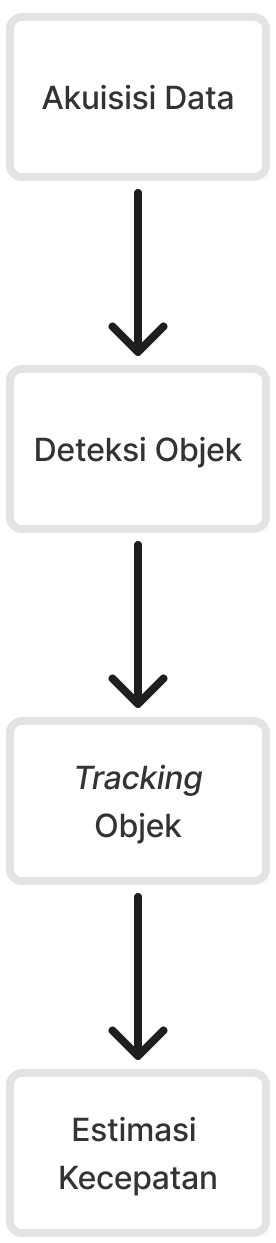
\includegraphics[scale=0.45]{bab3/diagramsistem.jpg}
  \caption{Diagram Alur Kerja Sistem}
  \label{fig:diagramsistem}
\end{figure}

Dilakukan akuisisi data untuk mengumpulkan dan melatih data yang diperoleh untuk proses deteksi objek. Untuk lebih akurat lagi, digunakan \emph{tracking} objek supaya dapat fleksibel mengikuti gerakan kendaraan. Pengukuran estimasi kecepatan dilakukan dengan menghitung perpindahan piksel antar \emph{frame} terhadap waktu.

\section{Akuisisi Data}
Tahap pertama yang diperlukan adalah mengumpulkan data melalui rekaman citra video dari kamera yang terpasang pada \emph{drone} hingga tahap melatih data yang diperoleh. Akuisisi data ini merupakan hal krusial karena sangat memengaruhi dari keberhasilan tahap selanjutnya seperti deteksi objek, dan \emph{tracking} objek. Berikut diagram blok dari alur akuisisi data yang dapat dilihat pada Gambar \ref{fig:akuisisidata} yang diproses sedemikian rupa sehingga data dapat digunakan untuk tahap selanjutnya.

\begin{figure} [H] \centering
  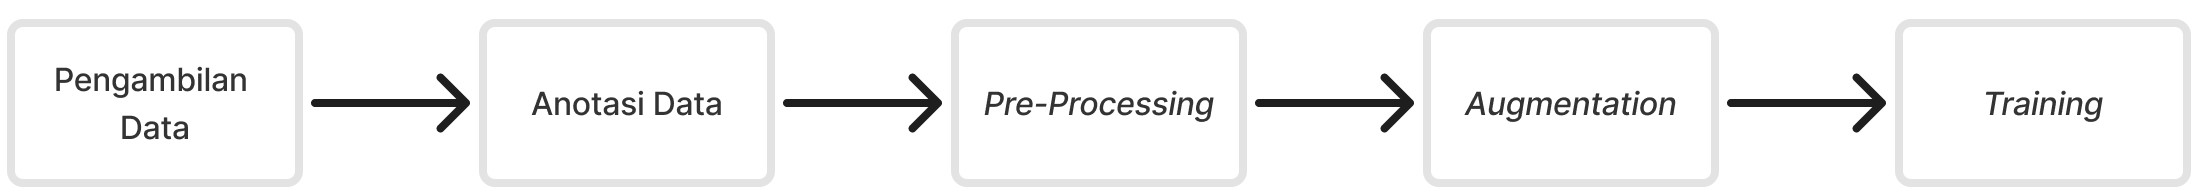
\includegraphics[scale=0.35]{bab3/akuisisidata.jpg}
  \caption{Diagram Blok Akuisisi Data}
  \label{fig:akuisisidata}
\end{figure}

%Section:Akuisisi Data%
\subsection{Pengambilan Data}
Data yang diambil merupakan hasil citra dari rekaman video yang diambil menggunakan kamera pada \emph{drone} dengan posisi \emph{birds view}, yang mana citra tampak dari atas. Salah satu data yang telah diambil dapat dilihat pada Gambar \ref{fig:datacitra_siang}, \ref{fig:datacitra_malam}.

\begin{figure} [H] \centering
  \includegraphics[scale=0.075]{bab3/citrasiang.jpg}
  \caption{Hasil Citra Pengambilan Data pada Siang Hari}
  \label{fig:datacitra_siang}
\end{figure}

\begin{figure} [H] \centering
  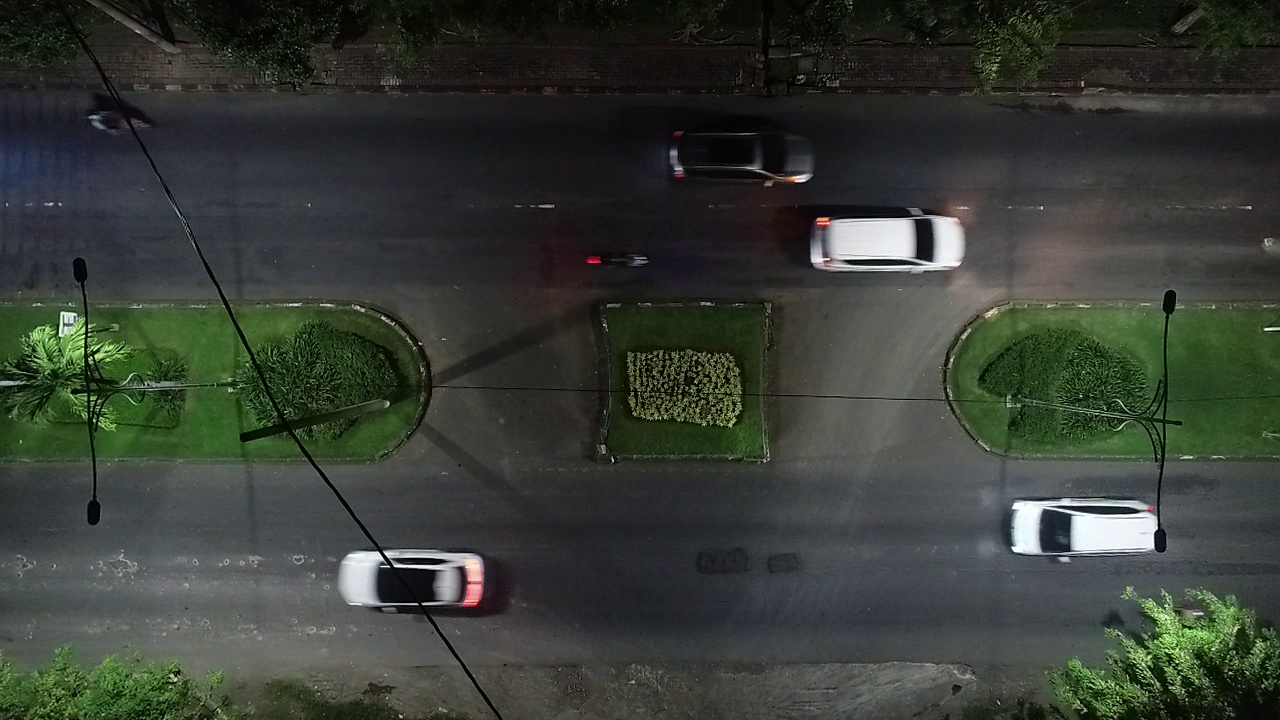
\includegraphics[scale=0.225]{bab3/citramalam.jpg}
  \caption{Hasil Citra Pengambilan Data pada Malam Hari}
  \label{fig:datacitra_malam}
\end{figure}

Citra tersebut diperoleh dari tiap frame yang diambil pada rekaman video \emph{drone} dari atas dengan kondisi siang hari dan malam hari. Pengambilan frame ini dilakukan secara komputasi dengan menjalankan sebuah program yang dirancang untuk mengambil setiap \emph{frame} citra dari video tersebut.

\subsection{Anotasi Data}
Setelah pengambilan data, hasil citra akan diberikan anotasi. Anotasi ini diberikan hanya pada objek yang akan dideteksi saja. Anotasi dilakukan dengan menggunakan \emph{tool} yang disediakan oleh Roboflow. Hasil anotasi dapat dilihat pada Gambar \ref{fig:anotasidatasiang} dan Gambar \ref{fig:anotasidatamalam}.

\begin{figure} [H] \centering
  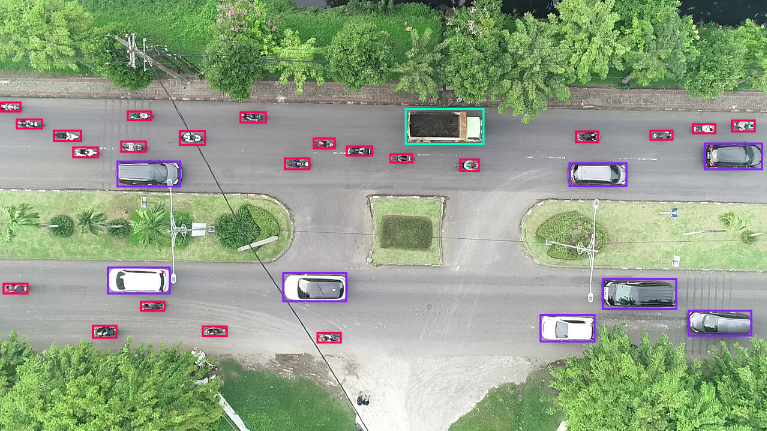
\includegraphics[scale=0.5]{bab3/anotasidatasiang.png}
  \caption{Citra Siang Setelah Dianotasi}
  \label{fig:anotasidatasiang}
\end{figure}

\begin{figure} [H] \centering
  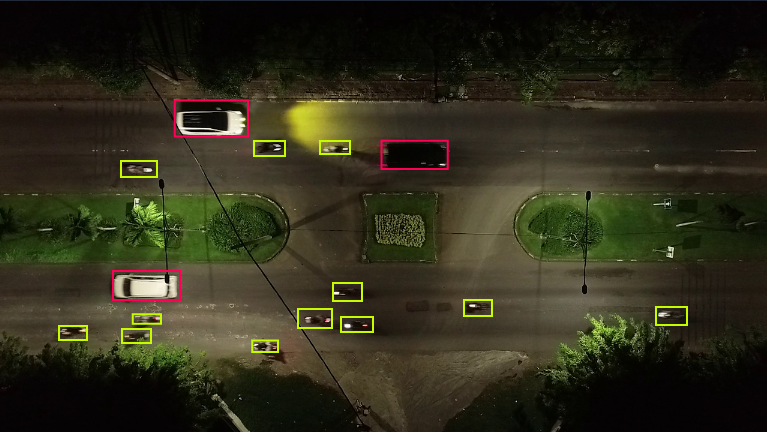
\includegraphics[scale=0.5]{bab3/anotasidatamalam.png}
  \caption{Citra Malam Setelah Dianotasi}
  \label{fig:anotasidatamalam}
\end{figure}

Objek diberi anotasi antara lain, mobil, motor, dan truk. Setelah anotasi selesai pada semua citra data, maka data dapat diubah menjadi sebuah dataset yang siap dilatih sehingga membentuk model deteksi objek.

\subsection{\emph{Pre-Processing}}
Proses ini merupakan persiapan dan transformasi data yang diperlukan untuk memudahkan saat \emph{training} serta proses analisisnya. \emph{Pre-processing} yang dilakukan pada data ini antara lain, \emph{auto-orient} dan \emph{resize} menjadi 320x320. Dua langkah tersebut diperlukan untuk mendapatkan performa \emph{training} yang lebih baik dan akurat.

\subsection{\emph{Augmentation}}
Pembuatan contoh pelatihan data baru untuk model yang dijalankan dari beberapa versi augmentasi setiap citra yang menjadi dataset. \emph{Augmentation} dapat membuat dan menambah variasi baru sehingga menambah citra data yang mana akan meningkatkan keakuratan dari model deteksi objek hasil \emph{training}. Beberapa augmentasi yang dilakukan adalah variasi \emph{flip}, rotasi 90 derajat, \emph{hue}, dan kecerahan.

\subsection{\emph{Training}}
Setelah dataset menjalani \emph{pre-processing} dan \emph{augmentation}, maka akan dilakukan pelatihan model deteksi objek dengan YOLOv8 yang merupakan \emph{framework} yang dikembangkan oleh Ultralytics. Proses \emph{training} ini akan belajar memahami pola dan mengenali objek yang dideteksi pada citra data. Model akan mengalami \emph{epoch} yang dapat diatur jumlah siklus sesuai kebutuhan. \emph{Epoch} merupakan siklus yang diproses untuk melatih model dengan setiap contoh maupun sampel dataset yang telah diproses sebelumnya. Model akan belajar mengenali objek dengan mengurangi \emph{loss} yang dihasilkan, dimana \emph{loss} merupakan jumlah banyaknya perbedaan yang dihasilkan dari prediksi model dengan anotasi yang sudah diatur. 

Pelatihan dilakukan dengan jumlah epoch sebanyak 250, dan saya atur menjadi \emph{half=True} (fp16). \emph{Batch size} diatur 18, dan \emph{workers} menjadi 18. Setelah didapatkan model (.pt) dari hasil pelatihan, diubah menjadi format onnx kemudian dikonversikan ke TensorRT. Proses \emph{training} ini menggunakan perangkat keras dengan spesifikasi yang dapat dilihat pada Tabel \ref{tbl:specpc}.

  \begin{table}[h!]
    \centering
    \captionof{table}{Tabel Spesifikasi Perangkat \emph{Training}}
    \label{tbl:specpc}
    \begin{tabular}{|c|c|}
      \hline
      \rowcolor[gray]{0.9}
      \textbf{\emph{Hardware}} & \textbf{Spesifikasi} \\ \hline
      CPU               & Intel Core i9 13900K \\ \hline
      GPU               & Nvidia Geforce RTX 4090 \\ \hline
      RAM               & 64 GB \\ \hline
    \end{tabular}
  \end{table}
 
\section{Deteksi Objek}
Deteksi objek dilakukan dengan menggunakan kamera \emph{drone} DJI Phantom 4 Pro dengan resolusi 720p dan 30 fps. Hasil tangkapan dari \emph{drone} akan dikirim melalui \emph{streaming} RTMP yang akan diterima oleh Jetson Nano untuk dilakukan pendeteksian objek dengan model YOLOv8 yang sudah dikonversi ke TensorRT.

Deteksi objek dilakukan pada sebuah video yang dikirim melalui \emph{stream} RTMP. Dari \emph{streaming} tersebut, akan diterima hasil tangkapan dari kamera drone yang kemudian diubah ke 360p untuk melakukan efisiensi pemrosesan oleh Jetson Nano. Lalu, beberapa objek yang menjadi fokus deteksi, antara lain mobil, motor, dan truk akan terdeteksi sesuai dengan objek yang melintas dan tertangkap kamera drone. Pendeteksian ini dijalankan dengan menggunakan model YOLOv8 yang telah dikonversi menjadi TensorRT untuk mendukung kapabilitas pendeteksian di Jetson Nano. Objek yang terdeteksi akan diberi label dan \emph{bounding box} sesuai dengan kelasnya. \emph{Bounding box} dan label ini akan menunjukkan objek apa yang ada didalam video tersebut. Pada Gambar \ref{fig:deteksi objek} dapat dilihat hasil deteksi objek yang dilakukan dengan model YOLOv8 dengan format TensorRT.

\begin{figure} [H] \centering
  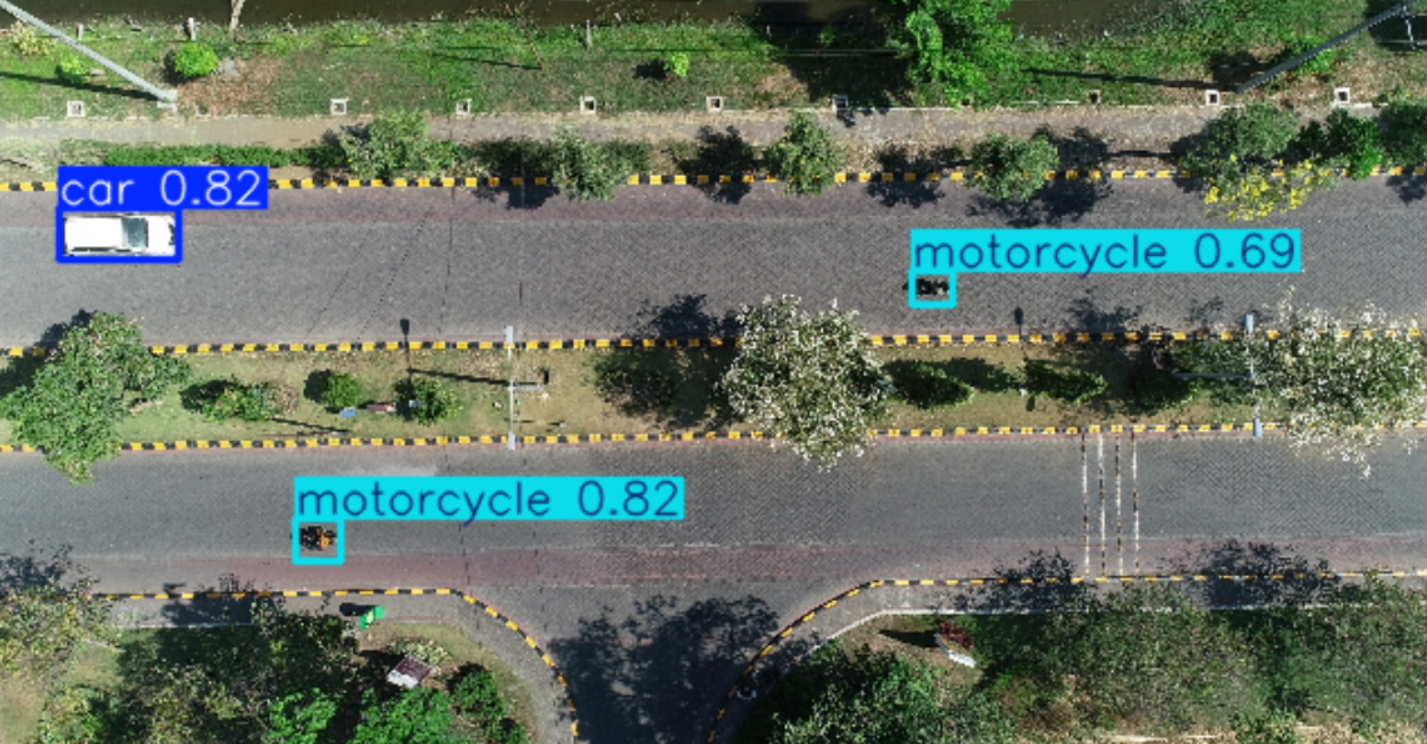
\includegraphics[scale=0.3]{bab3/deteksiobjek.png}
  \caption{Hasil Deteksi Objek}
  \label{fig:deteksi objek}
\end{figure}

Hasil implementasi deteksi objek pada video menggunakan model YOLOv8 yang sudah dilatih dan dikonversi menjadi TensorRT ditunjukkan pada Gambar \ref{fig:deteksi objek}. Pada Gambar \ref{fig:deteksi objek} didapatkan \emph{confidence threshold} diatas 0.5, dikarenakan deteksi objek yang dilakukan diatur untuk membaca objek yang memiliki \emph{confidence threshold} diatas 0.45 lalu memberi \emph{bounding box} pada objek yang terdeteksi.

\section{\emph{Tracking} Objek}
Pada tahap ini, objek akan dilakukan \emph{tracking} setelah terdeteksi. Untuk algoritma \emph{tracking} yang digunakan adalah OC-SORT dan ByteTrack. Dari dua metode \emph{tracking} tersebut terdapat perbedaan yang signifikan pada penelitian yang dilakukan dimana ByteTrack lebih cepat pemrosesannya daripada OC-SORT tetapi mengorbankan akurasi lebih banyak. Maka, metode OC-SORT yang digunakan dalam \emph{tracking} di penelitian ini.

Untuk perhitungan \emph{center} dalam penentuan \emph{bounding box} nya menggunakan persamaan titik tengah dalam geometri analitik, dengan menjumlahkan koordinat pojok sehingga ditemukan titik tengah dari objek deteksi setiap \emph{frame} dan diberi ID unik beserta nama \emph{class} sesuai dengan jenis objek yang terdeteksi.

\section{Estimasi Kecepatan}
Pada proses ini, objek yang telah terdeteksi dan menghasilkan \emph{bounding box} akan diukur kecepatannya. Dilakukan perhitungan titik tengah dengan menggunakan persamaan Euclidean yang dapat dilihat pada rumus \ref{eq:euclidean}.

\begin{equation}
  \label{eq:euclidean}
  \text{Jarak} = \sqrt{(x_2 - x_1)^2 + (y_2 - y_1)^2}
\end{equation}

\begin{flushleft}
Dimana:
\begin{align*}
x_1 & : \text{Koordinat $x$ titik pertama} \\
y_1 & : \text{Koordinat $y$ titik pertama} \\
x_2 & : \text{Koordinat $x$ titik kedua} \\
y_2 & : \text{Koordinat $y$ titik kedua} \\
\text{Jarak} & : \text{Jarak Euclidean antara dua titik}
\end{align*}
\end{flushleft}

Kemudian objek yang terdeteksi akan bergerak sehingga perpindahannya dihitung dengan selisih titik tengah. Hasil selisih tersebut akan dilakukan pembagian dengan \emph{Pixels per Meter} (PPM) yang didapatkan dari Persamaan \ref{eq:gsd_full}, setelah itu dikonversikan dimana hasilnya berbentuk cm/piksel menjadi piksel per meter. Berikut adalah hasil skala yang didapatkan untuk setiap ketinggian yang dijadikan variabel penelitian. 

\begin{table}[h!]
  \centering
  \captionof{table}{Hasil Skala Meter per Piksel}
  \label{tbl:skala_ppm}
  \begin{tabular}{|c|c|}
    \hline
    \rowcolor[gray]{0.9}
    \textbf{Ketinggian (m)} & \textbf{Meter per Piksel} \\ \hline
    20                      & 1 : 21,44                 \\ \hline
    30                      & 1 : 14,30                 \\ \hline
    40                      & 1 : 10,72                 \\ \hline
  \end{tabular}
\end{table}

Setelah itu, dilakukan perhitungan estimasi kecepatan dengan persamaan \ref{eq:speed_ms}.

\begin{equation}
  \label{eq:speed_ms}
  \text{Kecepatan(m/s)} = \frac{\text{Jarak(m)}}{\text{Waktu(s)}} \times 3{,}6
\end{equation}

\begin{flushleft}
Dimana:
\begin{align*}
Jarak & : \text{Jarak perpindahan objek deteksi} \\
Waktu & : \text{Waktu yang dibutuhkan objek deteksi berpindah} \\
\text{Kecepatan} & : \text{Hasil perhitungan kecepatan dalam satuan (m/s)}
\end{align*}
\end{flushleft}

Dikarenakan kecepatan kendaraan yang tertera pada \emph{speedometer} menggunakan satuan (\emph{km/h}) sehingga diperlukan untuk diubah satuan nya menjadi (m/s) seperti pada persamaan \ref{eq:speed_ms}.

\section{Penggunaan Alat}
Perangkat komputasi yang digunakan adalah Jetson Nano. Jetson Nano akan dikoneksikan ke \emph{controller drone} melalui protokol RTMP(\emph{Real-Time Streaming Protocol}). IP akan dikonfigurasikan antara Jetson Nano dengan \emph{drone} pada jaringan yang sama sehingga Jetson Nano dapat menerima hasil \emph{streaming}. Pembuatan \emph{server} RTMP sendiri menggunakan MediaMTX, kemudian \emph{drone} akan mengirim \emph{stream} ke \emph{server} tersebut, sehingga Jetson Nano akan membaca \emph{stream} menggunakan \emph{library} FFmpeg. Alur pengiriman data dapat dilihat pada Gambar \ref{fig:alurdata}.

\begin{figure} [H] \centering
  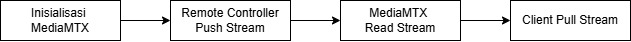
\includegraphics[scale=0.7]{bab3/pengirimandata.jpg}
  \caption{Diagram Alir Pengiriman Data}
  \label{fig:alurdata}
\end{figure}

Untuk algoritma yang digunakan dalam program estimasi ini terdapat beberapa tahapan yang harus dilewati sehingga program dapat berjalan sesuai. Diagram proses algoritma program ditunjukkan pada Gambar \ref{fig:diagramproses}.

\begin{figure} [H] \centering
  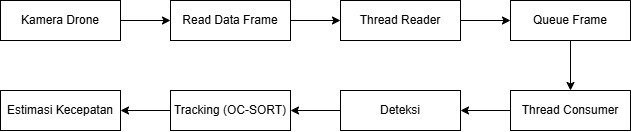
\includegraphics[scale=0.7]{bab3/algoritma.jpg}
  \caption{Diagram Alir Pemrosesan Data}
  \label{fig:diagramproses}
\end{figure}

Dalam menjalankan program estimasi ini tentu diperlukan perangkat keras untuk melakukan pemrosesannya. Perangkat keras yang digunakan dalam penelitian ini, antara lain \emph{drone}, \emph{smartphone}, laptop, Jetson Nano. Topologi perangkat keras yang digunakan dapat dilihat pada Gambar \ref{fig:topologihardware}.

\begin{figure} [H] \centering
  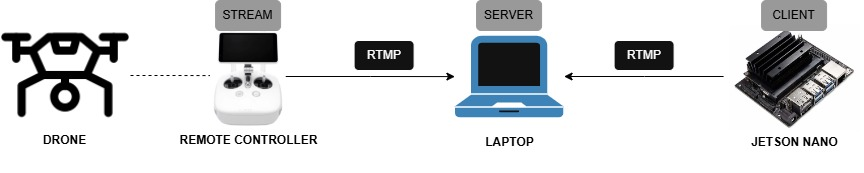
\includegraphics[scale=0.5]{bab3/topologi-hardware.jpg}
  \caption{Topologi Perangkat Keras}
  \label{fig:topologihardware}
\end{figure}

Pada Gambar \ref{fig:topologihardware} dapat dilihat bahwa RTMP sangat berperan penting dalam menghubungkan \emph{drone} dengan Jetson Nano sehingga hasil video yang direkam oleh \emph{drone} dapat dibaca langsung oleh Jetson Nano, dan dikomputasi juga pada Jetson Nano. Perangkat ini dibuat supaya komputasi dan visualisasi dapat dimodifikasi langsung di tempat sehingga lebih \emph{portable}.





